\section{Application Experience}\label{sec:application}

The application experience focuses on supporting the user in a building modeling task. The exploited modeling approach requires the user to face as much as possible a two-dimensional interface which allows her to define the plan and to place complex architectural elements (here called \emph{building elements}) on it. Such \emph{building elements} can be found in a pre-filled catalog, and when required can be further configured and customized through a side panel. This modeling approach move part of the complexity toward the developer of the customizable building elements, leaving to the final user the task to place and to configure the employed elements. A rich catalog of elements is thus crucial to answer to the users' modeling requirements.

Once the floor-plan has been defined according to the \emph{place-and-configure} approach, the system can automatically generate a 3D model which can be explored externally or in first person view, as shown in Figure~\ref{fig3D-school}. Each  \emph{building element} in fact comprises either a \emph{2D generating function (2dgf)} and a \emph{3D generating function (3dgf)}, used to obtain models used in the 2D floorplan definition and in 3D generated model respectively.

The tool also has support for layers the user can exploit to organize her project, for example to group together semantically homogenous elements.

\subsection{Building Elements}\label{ssec:elements}

Along with the aforementioned 2D and 3D generating functions, an elements is fully specified by its univocal name and its properties, used by the user for customization. Each building element inherits from its \emph{prototype} (one and only one). The prototype maps both the inherent characteristics and user interactions needed to add the element to the project and/or configure it.

The catalog comprises then four different types of elements:\\\\
\noindent \emph{Lines}. An element which belongs to this category is drawn selecting a start point and an end point. To move it one can drags one of the end-points or can drags the entire line. An example: a \emph{wall}.\\\\
\noindent \emph{Openings}. An opening is an element that is linked to a line-element, making an ``hole'' on it. The user creates a new opening by dragging an opening-element on a chosen line-element. Examples are \emph{doors} and \emph{windows}.\\\\
\noindent \emph{Areas}. An area is an element which may be generated by defining the boundary vertices. A \emph{room basement} is a good example of an area-element, which is automatically generated from walls (that are line-elements). The algorithm for the basement computation follows these phases: (i) search of biconnected component by mean of Hopcroft-Tarjan algorithm~(see \cite{Hopcroft:1973:AEA:362248.362272}); (ii) removal of edges that are not part of a biconnected component; (iii) search of all cycles through an algorithm that do a double check of each edges sorted by angle; (iv) search of maximal cycles correspondent to perimeter edges by an application of Gauss's area formula; (v) removal of maximal cycles.\\\\
\noindent \emph{Object}. An element that is freely inserted into space with a drag and drop interaction. Examples are \emph{tables} and \emph{chairs}.\\\

% The internal representation for Line types (e.g. walls) is undirected graph: each node maps coordinates of one tip of the line, each edge represents topological adjacency between vertex. This internal representation helps us to provide a drag and drop interaction for this element type, in fact each drag is performed by means of a relocation od a node that cause, other that the displacement of the requested wall, a displacement of each adjacent wall.


% Areas are automatically generated thanks to an analysis of the wall graph. The algorithm is composed by the following phases: (i) search of biconnected component by mean of Hopcroft-Tarjan algorithm~(see \cite{Hopcroft:1973:AEA:362248.362272}); (ii) removal of edges that are not part of a biconnected component; (iii) search of all cycles through an algorithm that do a double check of each edges sorted by angle; (iv) search of maximal cycles correspondent to perimeter edges by an application of Gauss's area formula; (v) removal of maximal cycles;


\subsection{User Interface}\label{ssec:ui}

\begin{figure}[htb]
\centering
\includegraphics[width=\linewidth]{contents/images/mock-interfaccia}
\caption{The user interface}
\label{figInterface}
\end{figure}

Figure~\ref{figInterface} shows the application user interface. It consists of the following components:

\emph{Content-area}: it displays the main content and it is chosen by the user. Developers can extend the available content-areas and so the functionalities of the system using techniques described in Section~\ref{sec:architecture}. Those which were already implemented by us are: (i) \emph{building elements catalog viewer} (figure~\ref{figCatalogo}), (ii) \emph{2D drawing area} (figure~\ref{fig2D}), (iii) \emph{3D viewer} (figures~\ref{fig3D-palace} and~\ref{fig3D}), (iv) \emph{3D first person viewer} (figure~\ref{fig3D-school})

\emph{Toolbar}: it contains buttons mapping all operations the user can do. Type and number of buttons change according to the content-area chosen

\emph{Sidebar}: it contains the list of building elements added to the current layer and the list of layers of the model. Moreover it permits to customize properties values for the selected elements\\

\begin{figure}[htb]
\centering
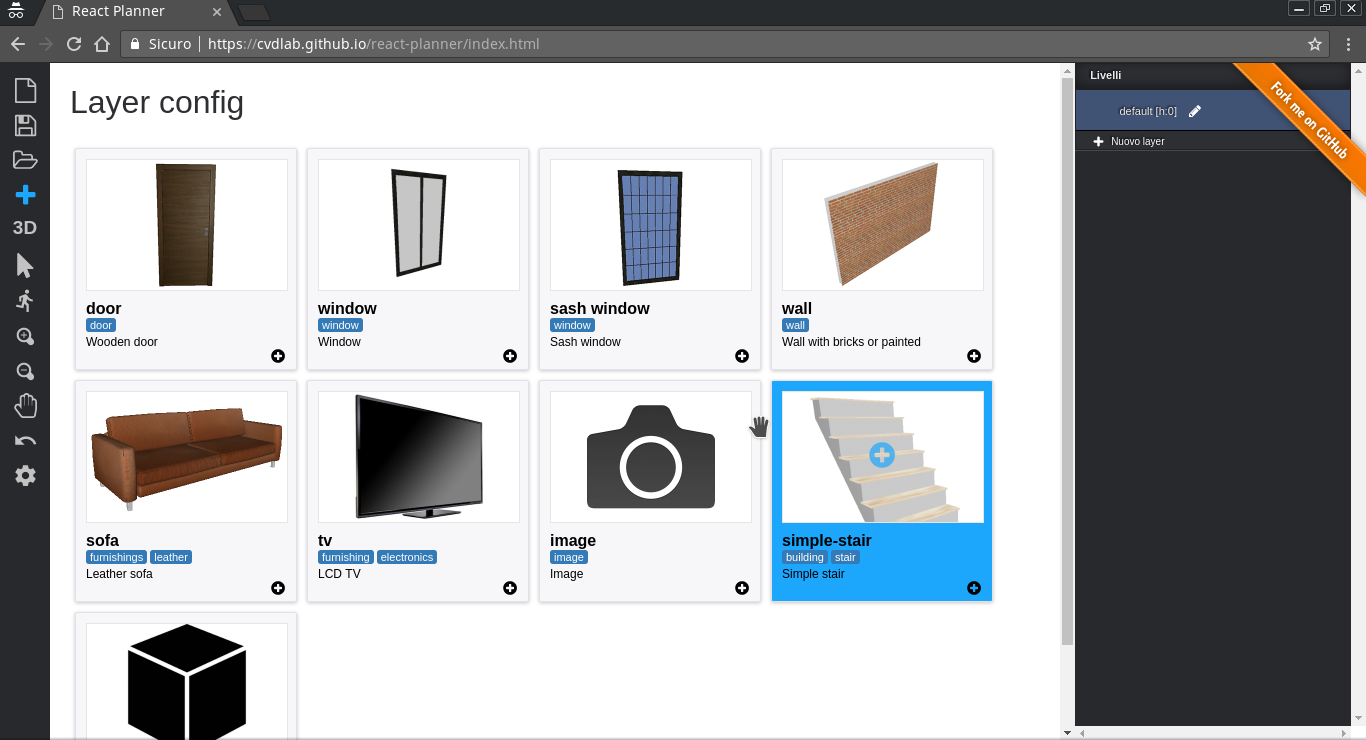
\includegraphics[width=\linewidth]{contents/images/figcatalog}
\caption{Building elements catalog}
\label{figCatalogo}
\end{figure}

\begin{figure}[htb]
\centering
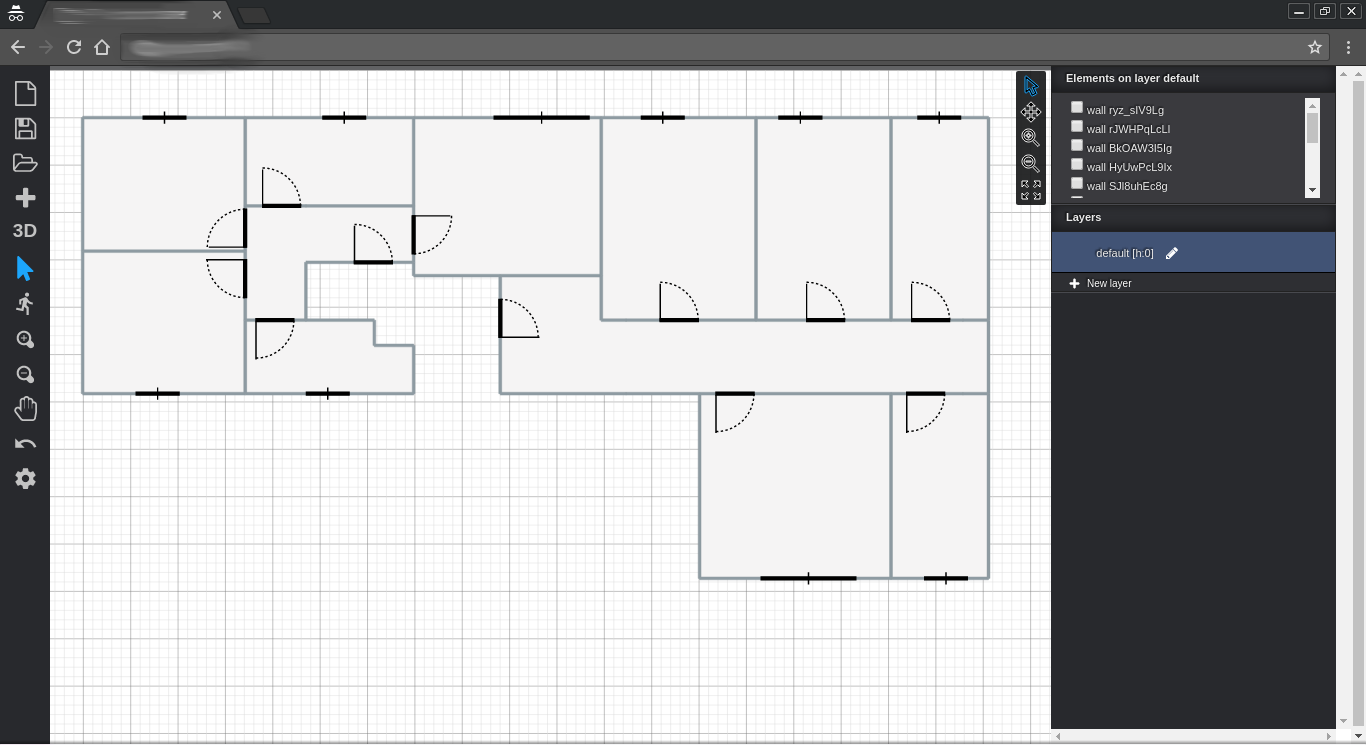
\includegraphics[width=\linewidth]{contents/images/fig-pianta}
\caption{The 2D drawing area}
\label{fig2D}
\end{figure}

\begin{figure}[htb]
\centering
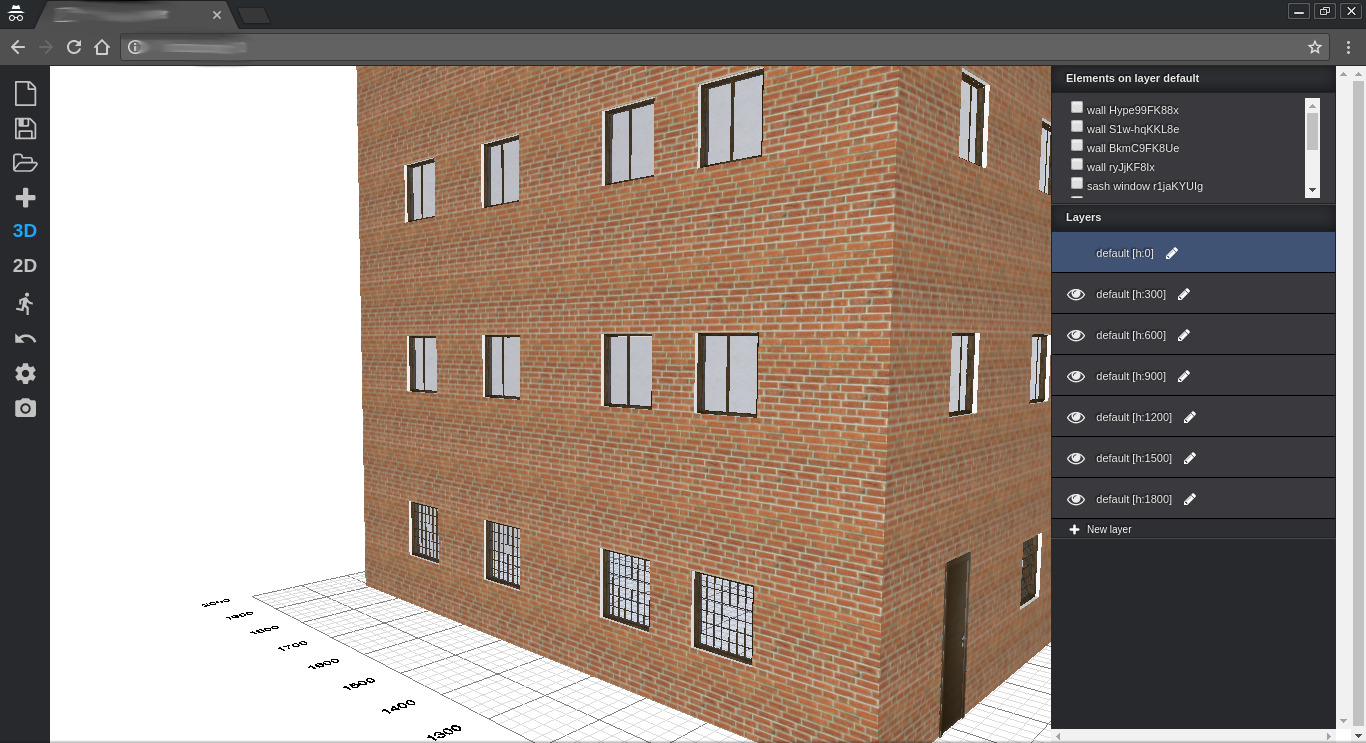
\includegraphics[width=\linewidth]{contents/images/palazzo2}
\caption{3D visualization of a building}
\label{fig3D-palace}
\end{figure}

\begin{figure}[htb]
\centering
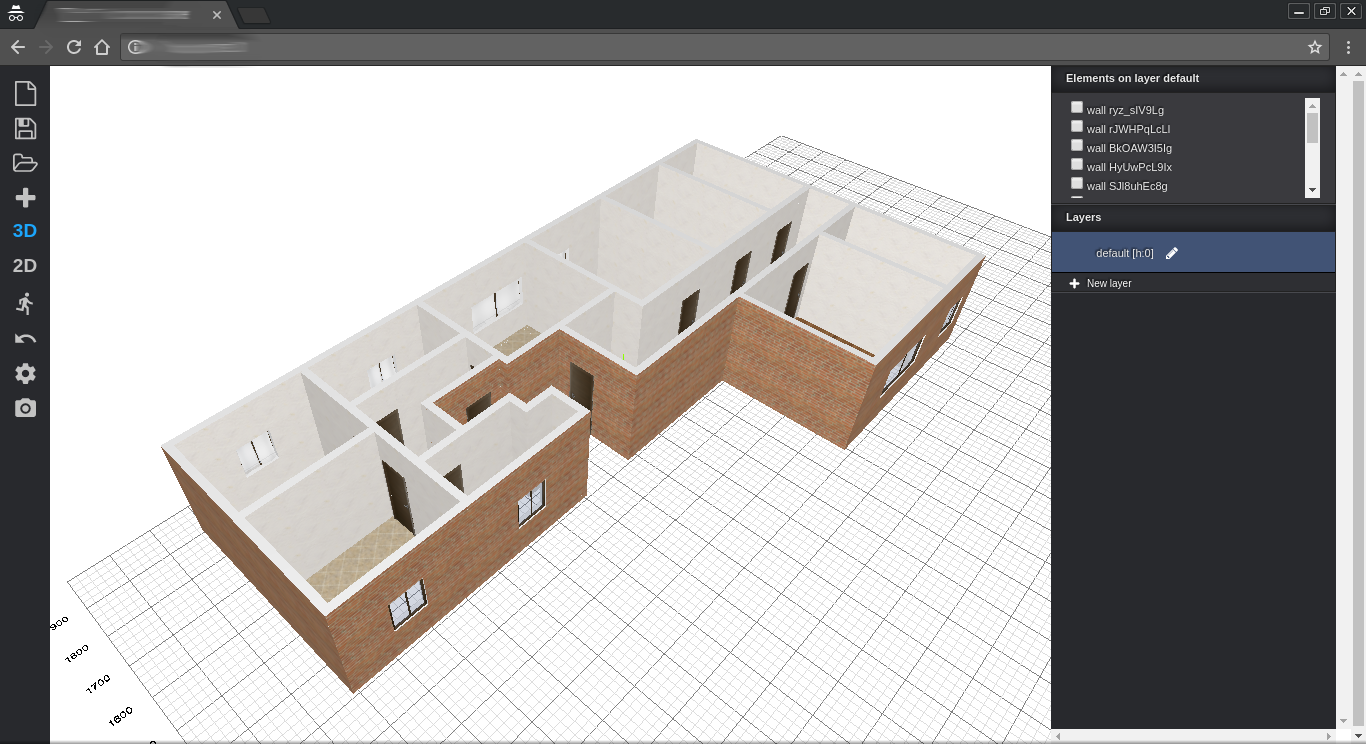
\includegraphics[width=\linewidth]{contents/images/fig-pianta-3d}
\caption{3D visualization for model in figure~\ref{fig2D}}
\label{fig3D}
\end{figure}

\begin{figure}[htb]
\centering
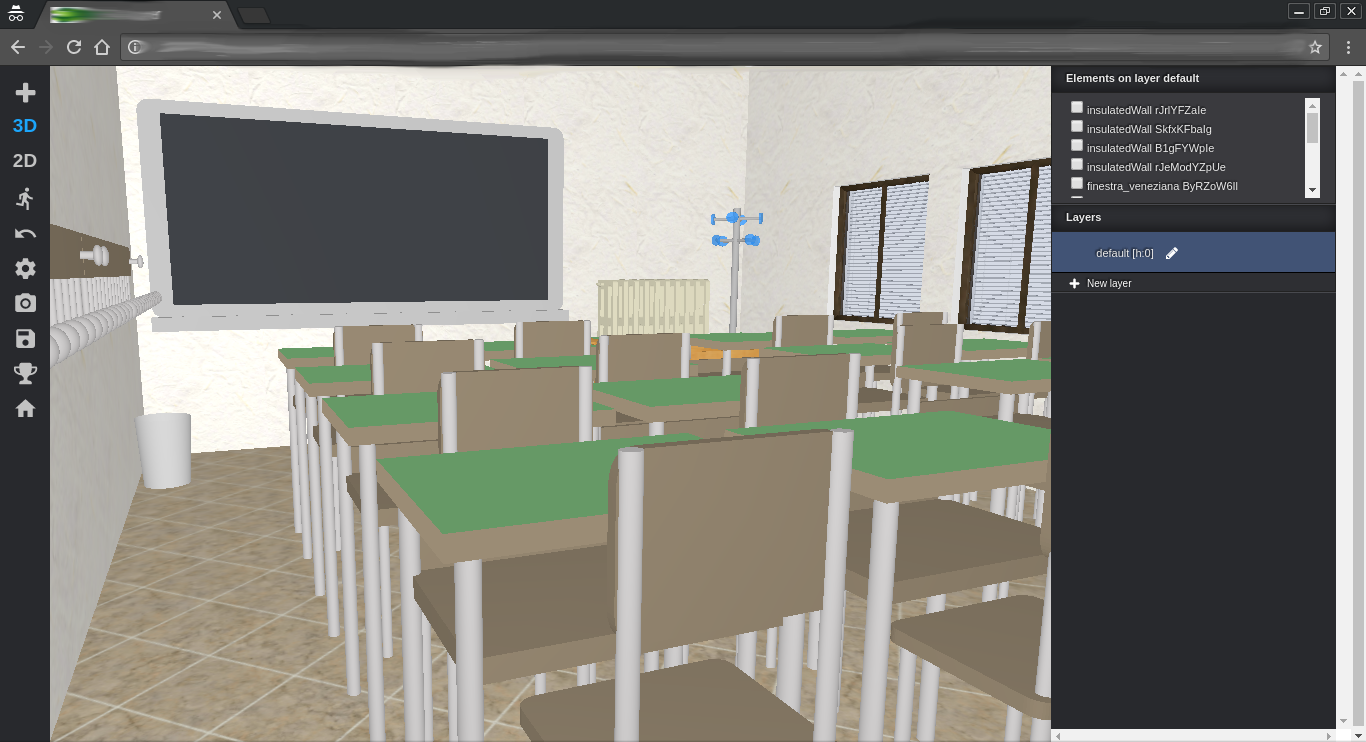
\includegraphics[width=\linewidth]{contents/images/3d-school}
\caption{3D first person walk-through inside a school model}
\label{fig3D-school}
\end{figure}